\chapter{Introduction}
\label{ch:intro}

A modern real-time material is not one image but several. A colour texture says what the
surface looks like under white light; a \emph{bump} or \emph{normal} map adds the small
dents and grooves that catch the light; a \emph{displacement} map really moves the surface;
and a \emph{roughness} map decides, point by point, whether the surface is glossy or dull.
Each of these maps is easy to describe in a sentence and surprisingly subtle to implement,
because it touches several ideas of computer graphics at once: the parametrization of
surfaces, the sampling of images, differential geometry, coordinate frames, and the physics
of reflection.

\emph{Texture Explorer} is a small interactive program written to make those ideas visible.
It shows a material and all its maps, applies them to a simple solid, and lets the student
move the camera and the light. Its central feature is a \emph{probe}: pointing with the mouse
at any texel of any map, the student sees
\begin{itemize}
\item the texture coordinates $(u,v)$ of the texel, normalized to $[0,1]$;
\item the value of every map there: colour, bump height, displacement and roughness;
\item the slope of the bump map, and the normal vector it implies, expressed both in the
\emph{tangent space} of the surface and in \emph{world} coordinates;
\item in the 3D view, the point of the solid that carries the texel, with arrows for the
geometric normal $\Nv$, the bumped normal $\vect n'$, and the tangent frame $\Tv$, $\Bv$.
\end{itemize}

\begin{figure}[ht]
  \centering
  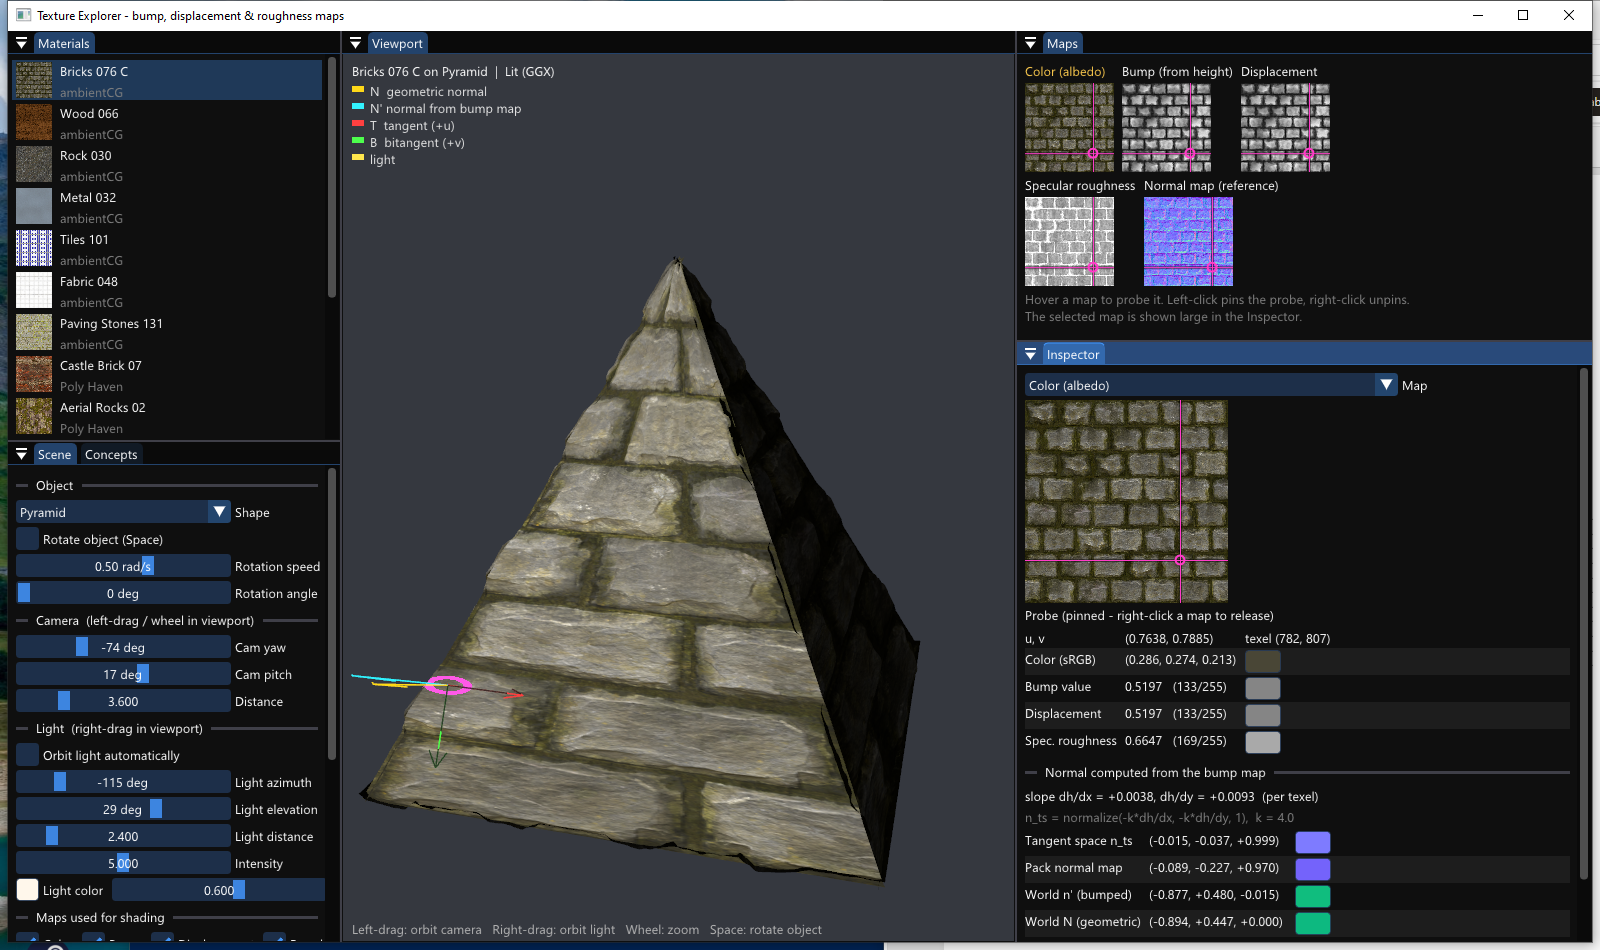
\includegraphics[width=\linewidth]{figures/pyramid-probe.png}
  \caption{Texture Explorer showing a brick material on the pyramid. The probe is pinned
  on a texel (crosshairs on every map); the Inspector lists its values and normals, and the
  3D view marks the same texel with a magenta ring and the arrows $\Nv$ (yellow),
  $\vect n'$ (cyan), $\Tv$ (red) and $\Bv$ (green).}
  \label{fig:pyramid}
\end{figure}

\section*{How this guide is organized}

Part~I develops the theory that the program illustrates. Chapter~\ref{ch:texspace}
introduces texture space and the parametrization of surfaces, using the four solids of the
program as examples. Chapter~\ref{ch:sampling} explains how a texture is sampled: texel
centres, bilinear filtering, mipmaps and colour spaces. Chapter~\ref{ch:height} is the core:
height fields used as bump maps and as displacement maps, the derivation of the perturbed
normal, and normal maps. Chapter~\ref{ch:tangent} studies the tangent frame and the
transformation of normals, and Chapter~\ref{ch:lighting} the microfacet model of reflection
through which roughness acts.

Part~II walks through the implementation. Every listing in it is extracted automatically
from the source files when this document is built, so the code shown is always the code that
runs; each listing is labelled with its file and line numbers. Chapter~\ref{ch:exercises}
proposes experiments and exercises for a course. For a broader treatment of every topic, see
the books by Akenine-M\"oller et al.\ \cite{akenine2018} and by Pharr et al.\ \cite{pharr2016}.

\section*{Running the program}

The program needs Windows 10 or later and a GPU with Direct3D~11. From the root of the
repository:

\begin{lstlisting}[language={},numbers=none,frame=none,basicstyle=\ttfamily\small]
powershell -ExecutionPolicy Bypass -File tools\fetch_textures.ps1   # once
cmake -S . -B build -G "Visual Studio 17 2022" -A x64
cmake --build build --config Release
build\Release\TextureExplorer.exe
\end{lstlisting}

The window is divided into dockable panels: \emph{Materials} (the list of materials and the
origin of the selected one), \emph{Scene} (controls), \emph{Concepts} (short explanations),
\emph{Viewport} (the 3D view), \emph{Maps} (all the maps of the material) and
\emph{Inspector} (the probe). In the viewport, dragging with the left button orbits the
camera, dragging with the right button orbits the light, the wheel zooms, and the space bar
starts or stops the rotation of the solid. On a map, hovering moves the probe, a left click
pins it, and a right click releases it.

\paragraph{Conventions.} Vectors are bold: $\vect p$, $\Nv$. Unit vectors are not marked
specially. The world is right-handed with $y$ up. Texture space follows Direct3D:
$(0,0)$ is the top-left corner of an image and $v$ grows downwards
(Section~\ref{sec:uvconv}).
